\documentclass[titlepage]{article}
\usepackage[T1]{fontenc}
\usepackage[utf8]{inputenc}
\usepackage{color}
\usepackage{hyperref}
\usepackage{float}
\usepackage{datetime}
\usepackage{graphicx}
\usepackage[margin=3cm]{geometry}
\graphicspath{{./assets}}
\hypersetup{
	colorlinks=true,
	linktoc=all,
	linkcolor=black,
}
	
\title{Typeracer Project Specification \\ \large Software Engineering 1}
\author{Muratcan Akçay, Kamil Monicz,\\ Maciej Piętka, Marcin Wojnarowski}
\date{\monthname, \the\year}
	
\newcommand{\secref}[1]{{(Section \hypersetup{linkcolor=blue}\ref{#1})}}

\newcommand{\figref}[1]{{(Fig. \hypersetup{linkcolor=blue}\ref{#1})}}

\begin{document}

\maketitle

\tableofcontents
\newpage

\section{Introduction}

\subsection{Preface}

It is without question that typing is a crucial skill in the age of computers. We type to message our loved ones, to write a professional email, to calculate, or even to write specifications such as this one. While other solutions such as Speech-To-Text are gaining popularity, they will never be able to replace typing. Typing serves as the primary mean of communication with our computers.

Often times the skill of typing is implicitly assumed by employers; nowadays nearly all jobs require some sort of interaction with a computer. Lack of this skill can greatly hinder our performance on a day to day basis.

Typing ranges from being a required chore to be able to communicate thoughts with a computer to a fun, competitive activity.

\subsection{Existing work}

Typing game is not an new idea, in fact the term {\it Typing game} is a popular video game genre. During the age of internet many new typing games have emerged. Below we present the current most popular choice for typing games and its drawbacks.

A homonymous site by the name of \url{typeracer.com} is by far the most popular choice for competitive and casual typing. Similarly to our project, {\it typeracer.com} focuses on real-time multiplayer. However, it comes with some important drawbacks:

\begin{itemize}
	\item Proprietary -- Source is not available, cannot be tinkered with

	\item Commercial model -- Some feature are locked behind a paywall

	\item Single client -- server-client communication is not standardized, forced to use the provided client

	\item Single server -- there is only one true server, games over the local network cannot be hosted
\end{itemize}

These limitations are the primary areas which will be directly tackled in this project.

\subsection{Overview}

The goal of the Typeracer project is to create a multiplayer interactive typing game. The aim is to create a standardized game server which will be able to host games for any compliant client regardless of its technological stack. The following three rules are to be enforced by the project:

\begin{enumerate}
	\item Clients are interchangeable and can coexist -- a server can host a game for any compliant client as well as different clients can be in the same game.

	\item Hostability -- server can be easily self hosted, whether that would be on a private server or on a local network.

	\item Real-time -- multiplayer games are updated in real time
\end{enumerate}

The game itself simply serves as a trainer and entertainer (if one enjoys fast typing). The game consists of a single input field, a text with the paragraph to be typed and the progress of all players \figref{fig:overview}.

\begin{figure}[ht]
	\centering
	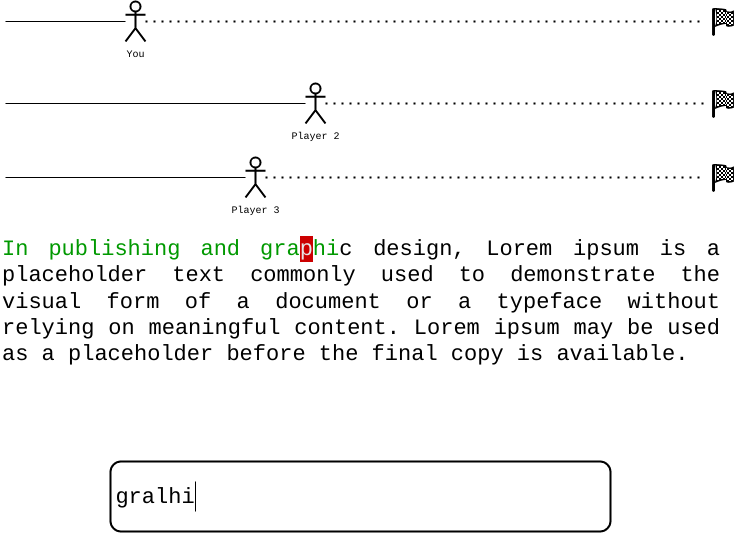
\includegraphics[width=0.79\textwidth]{overview.png}
	\caption{Overview of the game}
	\label{fig:overview}
\end{figure}

However before one can reach the game, the preferred game server has to be picked. Afterwards player waits in a lobby where other players can join the room. To help pass time, the lobby has an integrated chat.

Everything is managed by a running server and games can be moderated by admins. Best scores are kept in a leaderboard which it too can be moderated by an admin.

To sum up, this project consists of three components:

\begin{enumerate}
	\item Client -- Interacts with players, plays games
	\item Server -- Hosts games
	\item Admin panel -- Interacts with admins, manages games
\end{enumerate}

\subsection{Nomenclature} \label{nomenclature}

The following terms will be used throughout the specification, some come from the typing world and some from the technical one.

\begin{itemize}
	\item {\bf WPM} -- Words Per Minute, primary typing metric. Defines the average amount of correctly typed words per minute.

	\item {\bf Typer} -- Typeracer player.

	\item {\bf DNF} -- Did Not Finish, equivalent with disqualification.
\end{itemize}

\section{Requirements}

To start, a strict set of requirements has to be defined. The requirements are expressed in User Stories, a list of functional requirements, and finally other non-functional ones. Clearly defined requirements are crucial for a complete and cohesive system, which has to be the case in Typeracer due to its interchangeable nature.

\subsection{User Stories}

User Stories are written from the user's perspective (whether that would be a player or admin) and describe the expected results together with some acceptance criteria.

\subsubsection{Player user stories}

The most important actor is the player, after all all components are built with the player in mind. The following set of user stories will help illustrate what a user expects from the game.

\newcommand{\AC}{\subitem AC. }

\begin{enumerate}
	\item
	      As a player, I want to play a competitive typeracer game so that I can compare my typing skills against other people, increase my typing skills and have fun.
	      \AC
	      The game accepts multiple players together to type a block of text and race against each other and announces the order of completion.

	\item
	      As a player, I want to set my playerName so that other players can see my name on the leaderboard if I score a high score.
	      \AC
	      The game allows players to set their names and use them for displaying the leaderboard.

	\item
	      As a player, I want to see the daily and all-time high scores so that I can compare my skill level to the best players.
	      \AC
	      The game provides functionality to display the top ten daily/all-time scores in words per minute format.

	\item
	      As a player, I want to see how many players I’m playing against and the placement of all players during the game so that I can compare my skill position to the players I am playing with.
	      \AC
	      The game shows the player’s position during the game.

	\item
	      As a player, I want to see the placement of all players at the end of the game so that I can compare my skill level to the players I played with.
	      \AC
	      The game shows each player’s placement and score in words per minute format at the end of each game.

	\item
	      As a player, I want to choose which regional server I want to play on so that I will have the least latency during the game.
	      \AC
	      The game allows for choosing from three regional servers (NA, Europe, Asia) to play on at the beginning.

	\item
	      As a player, I want to chat with the other players after a game is over so that I can communicate with the other players and express my opinions.
	      \AC
	      The game displays a chat box at the end of each individual game where the players can chat until the next game begins.
\end{enumerate}

\subsubsection{Admin user stories}

The second actor is the admin which can moderate various aspects of the server and clients. The following list enumerates expectations of an admin with regards to their admin panel.

\begin{enumerate}
	\item
	      As an admin, I want to search the content database so that I can see which entries contain the search phrase I enter and remove that entry if I want.
	      \AC
	      The game allows admins to search the database and displays the entries containing the search phrase.

	\item
	      As an admin, I want to add or remove content to the game so that I have control over the texts that will be shown to the players.
	      \AC
	      The game allows admins to add or game content to the database by pasting in a text box or importing as a .txt file.

	\item
	      As an admin, I want to edit the displayed announcement text so that players are informed about important events such as server downtime or high score reset dates.
	      \AC
	      The game allows admins to modify the announcement text displayed on the main game window.

	\item
	      As an admin, I want to shut down the game service so that I can make changes in the configuration of the game without problems.
	      \AC
	      The game allows admins to shut down the game service.

	\item
	      As an admin, I want to restart the game service so that changes made can take effect and any existing errors can be remedied.
	      \AC
	      The game allows admins to restart the game service.

	\item
	      As an admin, I want to reset the leaderboard so that a new game season can be started with a blank all-time leaderboard allowing new players to compete for the high scores.
	      \AC
	      The game allows admins to reset the leaderboard.

	\item
	      As an admin, I want to adjust the queue duration so that I can manage how long players have to wait before a game starts.
	      \AC
	      The game allows admins to adjust the waiting queue duration.

	\item
	      As an admin, I want to adjust the DNF (did not finish) duration so that I can manage how long players have to wait before a game ends, even if one of the players never finishes typing the text.
	      \AC
	      The game allows admins to adjust the DNF duration.
\end{enumerate}

\subsection{Functional requirements}

To be more specific, a list of core functional requirements is listed below.

\begin{itemize}
	\item The players can set their player names before starting to play the game
	\item The players can see the daily and all-time leaderboards where high scores are displayed.
	\item While a game is being played, the players can see how many players are playing and their placement among other players in real-time.
	\item When a game ends the players can see their final placement among other players that participated in the game and their typing speed in wpm (words per minute).
	\item The players can choose which regional server they want to play on to mitigate the effects of latency.
	\item The admins can log in to the admin panel using an admin passphrase
	\item The admins can edit the announcement text which will be displayed to the players.
	\item The admins can shut down the game service
	\item The admins can restart the game service
	\item The admins can adjust the waiting queue duration that counts down before the start of each game
	\item The admins can adjust the did not finish duration that defines the max. Time a game will last
	\item The admins can view the content database to see the entries sorted by date added
	\item The admins can search the content database to find all entries containing a specific search phrase
	\item The admins can remove an entry from the database
	\item The admins can add an entry to the database by pasting the text in a text box or importing a .txt file
	\item The admins can reset the all-time leaderboards
\end{itemize}

\subsection{Non-Functional requirements}

Finally, a set of non-functional requirements has to be presented to further describe the vision.

\subsubsection{Usability}

\begin{itemize}
	\item The service is available in English, for all users with an Internet/LAN connection.
	\item The user interface for the players is minimalistic, allowing only keyboard input, clear and easy to use.
	\item The user interface for the admins is minimalistic, allowing both mouse and keyboard input, clear and easy to use.
\end{itemize}

\subsubsection{Reliability}

\begin{itemize}
	\item The service will have at max 5\% of downtime.
	\item The service will be logging any encountered errors.
	\item The service will be restored in maximum of 1 day after a fatal error.
\end{itemize}

\subsubsection{Performance}

\begin{itemize}
	\item The service will support at least 1000 concurrent players on each server.
	\item The service can be scaled to support more users at a time.
\end{itemize}

\subsubsection{Supportability}

\begin{itemize}
	\item Both the player and admin components of the system will only be web-based and run on latest versions of Chrome, Firefox and Microsoft Edge browsers.
\end{itemize}

\newpage

\subsection{Use case diagram}

To sum up the requirements in a visual form, which will give a rough idea of how the usage should flow.

\begin{figure}[ht]
	\centering
	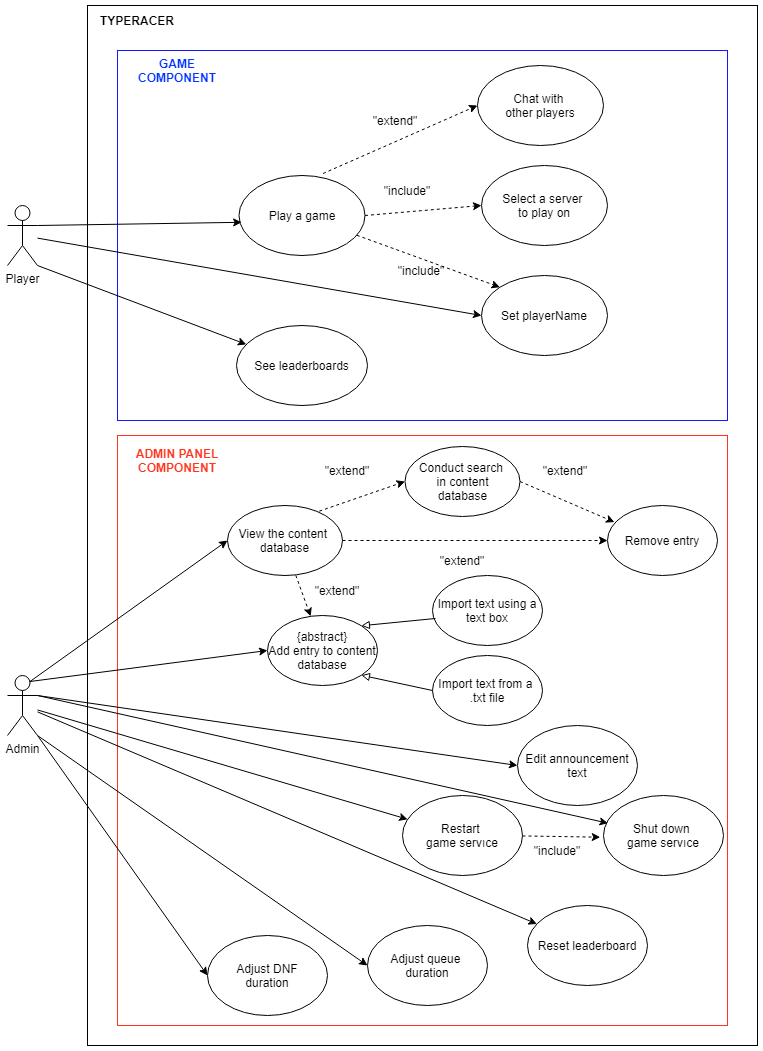
\includegraphics[width=0.75\textwidth]{use_case_diagram.png}
	\caption{Typeracer use case diagram}
	\label{fig:usecase-diag}
\end{figure}

\newpage

\section{Design}

In this section system's behavior and expected states are described.

\subsection{Class diagram}

The system can be split into few core components \figref{fig:class-diag}:

\begin{itemize}
	\item {\bf Player} -- It has to be able to select a server to which it will be able to later join a game. A player can also set its name as well as show the leaderboard.
	\item {\bf Chat} -- The chat module boils down to being able to send and receive messages.
	\item {\bf GameService} -- Manages starting and ending games. Additionally it can accept incoming connections and drop when needed. Whenever needed, it can also update the leaderboards.
	\item {\bf Lobby} -- Once players are in the lobby they are managed by the lobby class where the queue can be started. It can also control which component is being shown: announcement, chat, and leaderboard.
	\item {\bf Announcement} -- Can only be retrieved, or changed by the admin.
	\item {\bf Admin} -- Controls other services. It can start, stop, or restart the server. It can authenticate the admin by letting them login but also log out. Admin can also alter the dnf countdown, the queue countdown as well as change the announcement text. It can also inspect the leaderboard.
	\item {\bf Leaderboard} -- A leaderboard can either be daily or all time. Both of them can be modified: resetting to a clean slate, adding a record to a leaderboard and getting the leaderboard.
	\item {\bf ContentManager} -- Allows adding and deleting texts that will be typed by the players. Texts can be added either as a raw string or from a text file which will include many texts separated by some delimiter. Finally, it allows for picking a random text.
\end{itemize}

\begin{figure}[H]
	\centering
	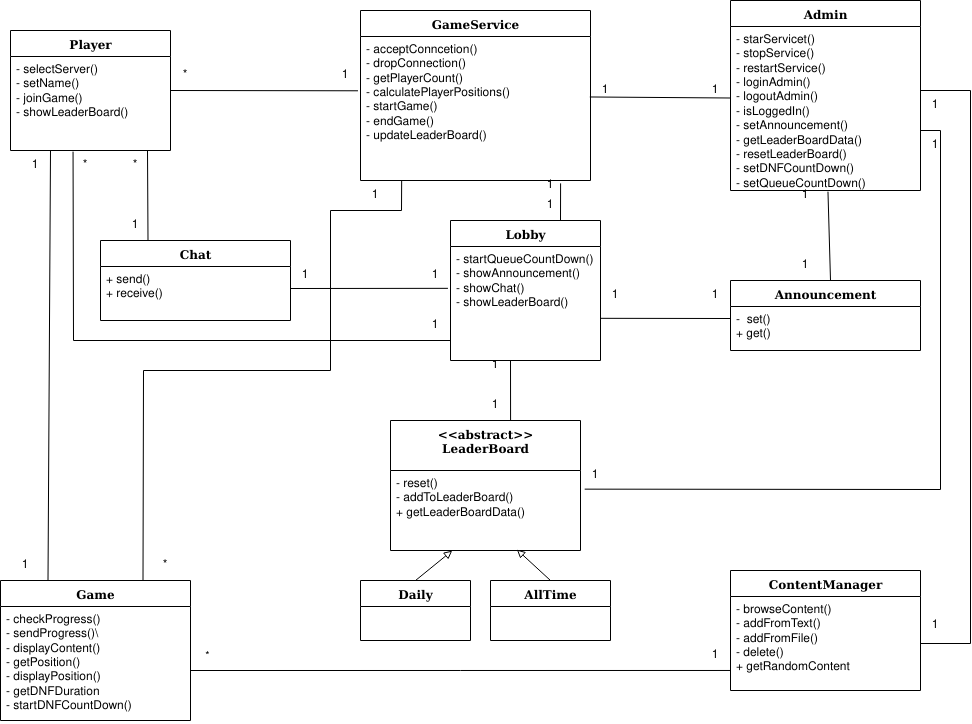
\includegraphics[width=0.79\textwidth]{class_diagram.png}
	\caption{Typeracer class diagram}
	\label{fig:class-diag}
\end{figure}

\subsection{State diagrams}

States of Typeracer are well defined, we can expect a fixed set of states.

\subsubsection{Server}

Server has a small amount of states \figref{fig:state-server}. Its responsibility is to accept incoming requests and handle them. Before receiving a request the server is in a waiting state. Once a request arrives it has to handle it, no matter whether the handling is successful or not, a response has to be sent back. In case of an error, it should be logged.

\begin{figure}[H]
	\centering
	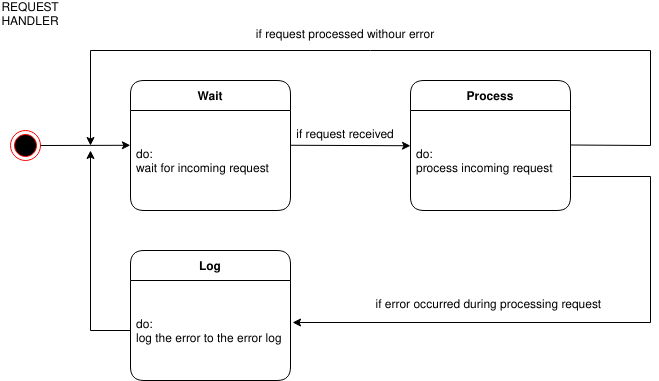
\includegraphics[width=0.79\textwidth]{state_diagram_server.png}
	\caption{Server's state diagram}
	\label{fig:state-server}
\end{figure}

\subsubsection{Admin panel}

Admin's state \figref{fig:state-admin} is the most complex due to the fact that many components can be altered resulting in many different states. The admin panel is guarded by a login screen which requires admin privileges. Once authorized, admin can browse many sub-pages in which they can change the behavior and look of the game. At any time, pressing the logout button brings the admin back to the login screen

\begin{figure}[H]
	\centering
	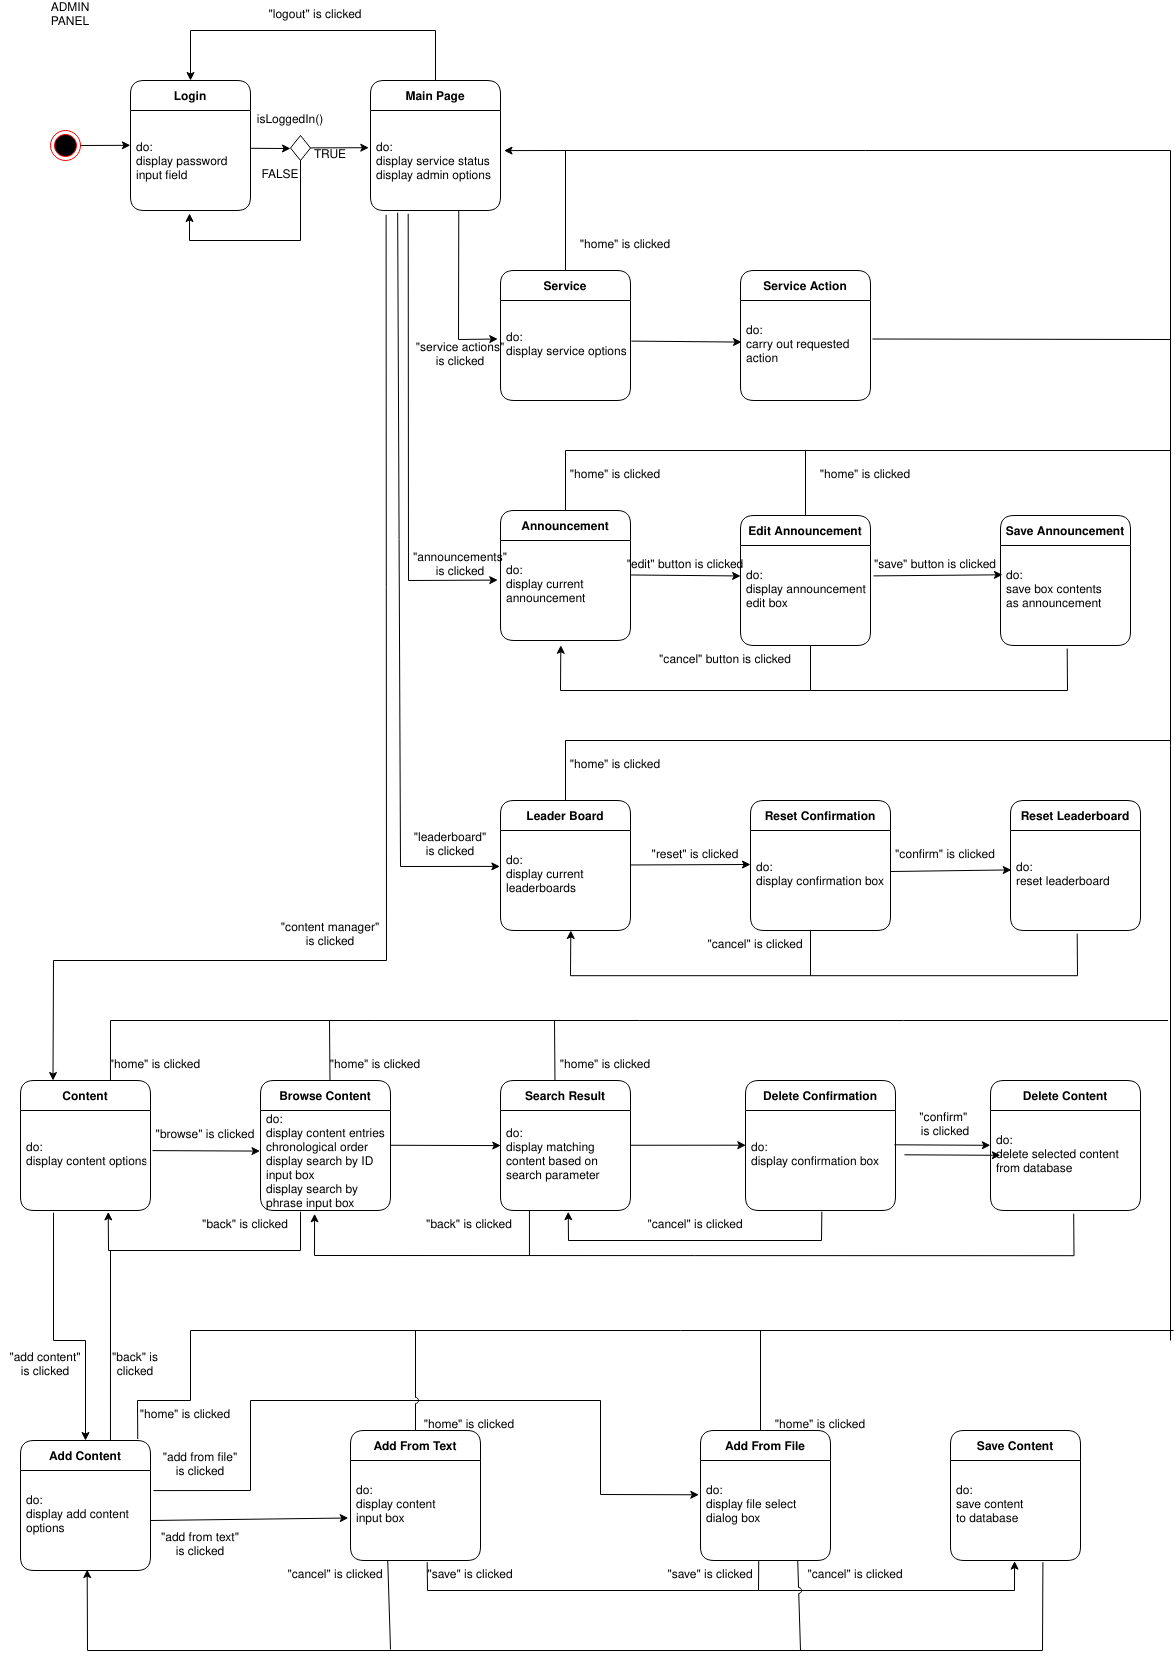
\includegraphics[width=0.79\textwidth]{state_diagram_admin.png}
	\caption{Admin's state diagram}
	\label{fig:state-admin}
\end{figure}

\subsubsection{Client}

Client's state is responsible for tracking player's progress and the usage flow. Three separate entities can be identified: Player, Lobby, and Game.

The player state \figref{fig:state-client-player} focuses on the states happening at the very beginning when the client is started. At first the user is prompted to enter their username, once it is confirmed and validated to be correct the user is redirected to a place where a game server can be chosen. Otherwise, the user stays in the set username screen until it is valid.

When selecting a server the only error state is a connection error. If it occurs the user is allowed to pick a game server again until success. Once a connection is successful user is moved to the lobby.

\begin{figure}[H]
	\centering
	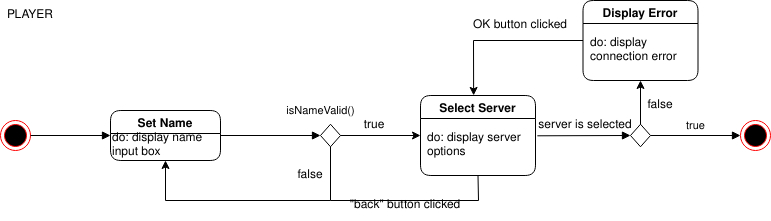
\includegraphics[width=0.79\textwidth]{state_diagram_player.png}
	\caption{Client's player state diagram}
	\label{fig:state-client-player}
\end{figure}

In the lobby \figref{fig:state-client-lobby} a countdown is ran in the background. Once it reaches zero, we exit the lobby and move to the game. Before that, there are two concurrent states: Lobby and Chat/Leaderboard. In the lobby the queue is displayed together with a announcement controlled by the admin. Chat and leaderboards are interchangeable and cannot be present at the same time. Leaderboards are spit into daily and all-time.

\begin{figure}[H]
	\centering
	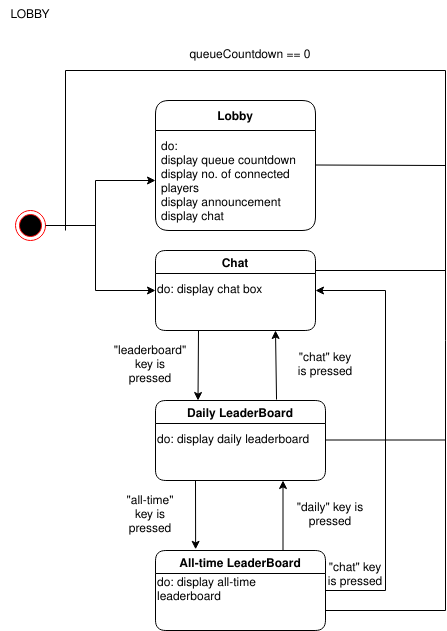
\includegraphics[width=0.79\textwidth]{state_diagram_lobby.png}
	\caption{Client's lobby state diagram}
	\label{fig:state-client-lobby}
\end{figure}

Finally, in the game section \figref{fig:state-client-game}, as the name suggests, the game takes place. Here the state is rather constant and is changed only if the game countdown reaches zero (which results in a DNF) or when every player finishes typing the text. During the game, the progress of other players is displayed, and the user advances through their text by typing consecutive words.

\begin{figure}[H]
	\centering
	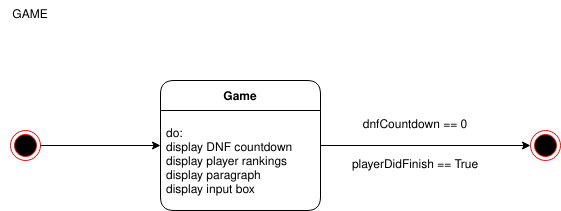
\includegraphics[width=0.79\textwidth]{state_diagram_game.png}
	\caption{Client's game state diagram}
	\label{fig:state-client-game}
\end{figure}


\end{document}
